\documentclass[a4paper, 12pt]{article}
\usepackage[utf8x]{inputenc}
\usepackage[english, russian]{babel}
\usepackage[left=25mm, top=25mm, right=25mm, bottom=25mm]{geometry}
\usepackage{cmap}
\usepackage{indentfirst}
\usepackage{tikz}
\usepackage{float}
\usepackage{amsmath, amsfonts, amssymb}
\usepackage{graphicx}
\usepackage{hyperref}
\usepackage{listings}
\usepackage{caption}
\usepackage{subcaption}
\usepackage{xcolor}
\usepackage{etoolbox}
\usepackage{titlesec}
\pagestyle{plain}
\patchcmd{\tableofcontents}{\contentsname}{\centering\contentsname}{}{}
\titleformat{\section}[block]{\normalfont\large\bfseries\centering}{}{0pt}{}
\titleformat{\subsection}[block]{\normalfont\normalsize\bfseries\centering}{}{0pt}{}
\allowdisplaybreaks
\graphicspath{{images/}}
\usetikzlibrary{patterns}
\definecolor{LightGray}{gray}{0.95}
\definecolor{LightGray2}{gray}{0.7}
\lstdefinestyle{code}{
    language=MATLAB, % replace language here
    basicstyle=\footnotesize\ttfamily,
    % numbers=left,
    % numberstyle=\scriptsize\color{gray},
    % stepnumber=1,
    % numbersep=5pt,
    backgroundcolor=\color{LightGray},
    showspaces=false,
    showstringspaces=false,
    showtabs=false,
    tabsize=4,
    captionpos=b,
    breaklines=true,
    breakatwhitespace=false,
    frame=single,
    rulecolor=\color{LightGray2},
    linewidth=\linewidth,
    keywordstyle=\color{blue}\bfseries,
    commentstyle=\color{green!40!black},
    stringstyle=\color{purple},
    escapeinside={\%*}{*)},
    inputencoding=utf8x,
    xleftmargin=0pt,
    framexleftmargin=0pt,
    framexrightmargin=0pt
}
\lstset{style=code}
\hypersetup{
    colorlinks=true,
    linkcolor=blue,
    filecolor=magenta,
    urlcolor=cyan,
    pdftitle={contents setup},
    pdfpagemode=FullScreen,
}


\begin{document}
    \begin{titlepage}

        \begin{center}
        Федеральное государственное автономное образовательное учреждение высшего образования
        «Национальный Исследовательский Университет ИТМО»
        \vfill
        
        
\includegraphics[width=0.3\textwidth]{itmo.png} % requires /images/itmo.png

        {\large\bf ЛАБОРАТОРНАЯ РАБОТА №2}\\
        {\large\bf ПРЕДМЕТ «ТЕОРИЯ АВТОМАТИЧЕСКОГО УПРАВЛЕНИЯ»}\\
        {\large\bf ТЕМА «МОДАЛЬНЫЕ РЕГУЛЯТОРЫ И НАБЛЮДАТЕЛИ»}\\
        Вариант №2
        \vfill

        \begin{flushright}
            \begin{minipage}{.45\textwidth}
            {
                \hbox{Преподаватель:}
                \hbox{Пашенко А. В.}
                \hbox{}
                \hbox{Выполнил:}
                \hbox{Румянцев А. А.}
                \hbox{}
                \hbox{Факультет: СУиР}
                \hbox{Группа: R3341}
                \hbox{Поток: ТАУ R22 бак 1.1.1}
            }
            \end{minipage}
        \end{flushright}
        \vfill
  
        Санкт-Петербург\\
        2025
        \end{center}
    \end{titlepage}
    
    \tableofcontents

    \newpage
    \section{Задание 1. Модальный регулятор}
    Рассмотрим систему
    $$
    \dot{x}=Ax+Bu,\ A=\begin{bmatrix}
        5 &2 &7\\
        2 &1 &2\\
        -2 &-3 &-4
    \end{bmatrix},\ B=\begin{bmatrix}
        3\\
        1\\
        -1
    \end{bmatrix},
    $$
    $$
    \sigma\left(A+BK\right)= 
    \left[ 
      \begin{gathered} 
        \left\{-2,-2,-2\right\}, \\ 
        \left\{-3,-3,-3\right\}, \\
        \left\{-2,-20,-200\right\},\\
        \left\{-3,-30,-300\right\},\\
        \left\{-2,-2\pm6i\right\},\\
        \left\{-3,-3\pm9i\right\};
      \end{gathered} 
\right.
    $$

    
    \subsection{Управляемость и стабилизируемость спектра и системы}
    Найдем собственные числа матрицы $A$ с помощью \texttt{MATLAB} (программу см. листинг \ref{task1} в приложении 1)
    $$
    \det{\left[\lambda I-A\right]}=\begin{vmatrix}
        \lambda-5 &-2 &-7\\
        -2 &\lambda-1 &-2\\
        2 &3 &\lambda+4
    \end{vmatrix}=0,
    $$
    $$
    \sigma\left(A\right)=\left\{-2, 2\pm i\right\}
    $$
    $\lambda_1=-2<0$ асимптотически устойчивое, может быть неуправляемым. $\lambda_{2,3}=2\pm i$ имеют
    положительные действительные части -- неустойчивые, нужна управляемость. Определим управляемость
    собственных чисел через жорданово разложение (приведение комплексной формы к вещественной аналогично первой
    лабораторной работе)
    $$
    A=P_{re}J_{re}P_{re}^{-1}=\begin{bmatrix}
    -1    &0.5   &-1.5\\
    0         &0   &-1\\
    1         &0    &1
    \end{bmatrix}\begin{bmatrix}
    -2     &0     &0\\
     0     &2     &1\\
     0    &-1     &2
    \end{bmatrix}\begin{bmatrix}
    0     &1     &1\\
     2    &-1     &2\\
     0    &-1     &0
    \end{bmatrix},
    $$
    $$
    B_{Jre}=P_{re}^{-1}B=\begin{bmatrix}
        0     &1     &1\\
         2    &-1     &2\\
         0    &-1     &0
        \end{bmatrix}\begin{bmatrix}
            3\\
            1\\
            -1
        \end{bmatrix}=\begin{bmatrix}
        0\\
     3\\
    -1
    \end{bmatrix}
    $$
    Итого имеем
    $$
    J_{re}=\begin{bmatrix}
        -2     &0     &0\\
         0     &2     &1\\
         0    &-1     &2
        \end{bmatrix},\ B_{Jre}=\begin{bmatrix}
            0\\
         3\\
        -1
        \end{bmatrix}
    $$
    Все жордановы клетки относятся к различным собственным числам. Собственное число $\lambda_1=-2$ неуправляемое, так как первый элемент в матрице
    входных воздействий $B_{Jre}$ равен нулю. Остальные собственные числа управляемые.
    Следовательно, система не полностью управляема. Достаточное условие полной управляемости
    системы в нашем случае -- не равенство нулю первого и $\left[\text{второго или третьего}\right]$
    элементов матрицы $B_{Jre}$. Оно не выполняется. Так как все неустойчивые собственные числа
    управляемы, то система стабилизируема.


    \subsection{Схема моделирования системы, замкнутой регулятором}
    Построим схему моделирования системы $\dot{x}=Ax+Bu$, замкнутой регулятором $u=Kx$, используя \texttt{SIMULINK}
    \begin{figure}[H]
        \centering
        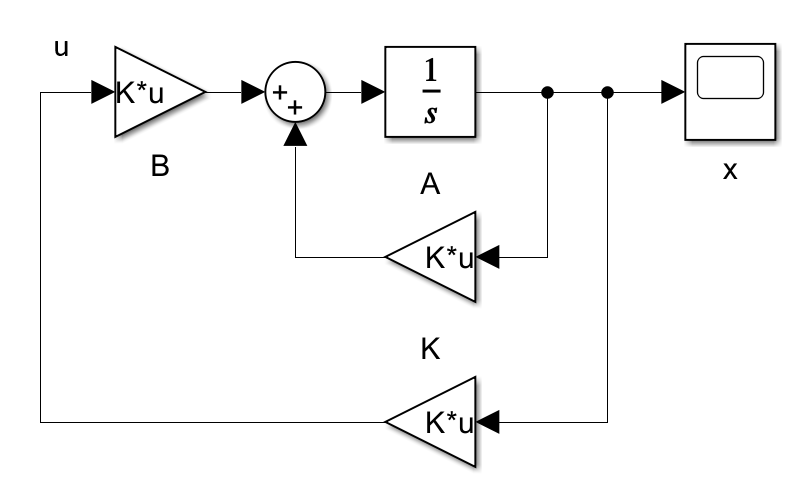
\includegraphics[scale=0.5]{scheme_task1.png}
        \captionsetup{skip=0pt}
        \caption{Схема моделирования системы, замкнутой регулятором}
        \label{fig:scheme_task1}
    \end{figure}


    \subsection{Достижимые спектры}
    Рассмотрим предложенные спектры замкнутой системы $\left(A+BK\right)$ и определим, какие из них достижимы.
    Мы хотим, чтобы матрица $\left(A+BK\right)$ была устойчивой, то есть все ее собственные числа имели
    отрицательную действительную часть. В нашем случае комплексная пара $\lambda_{2,3}$ являются неустойчивыми,
    но управляемыми -- их можно переместить в устойчивую область (подобрать любые числа, меньшие нуля). Собственное
    число $\lambda_1=-2$ устойчивое, но неуправляемое -- его не получится переместить куда-либо. Это означает, что
    спектр $\sigma\left(A+BK\right)$ должен содержать это неуправляемое число, иначе регулятор не будет выполнять свою
    функцию, мы потеряем собственное число матрицы $A$. Таким образом, желаемый спектр должен содержать все неуправляемые (но устойчивые)
    собственные числа матрицы $A$, при этом остальные числа могут быть любыми, но устойчивыми. Важно уточнить, что
    если некоторое собственное число матрицы $A$ неустойчиво и неуправляемо, то система не стабилизируема -- модальный
    регулятор применить не получится.


    Исходя из наших рассуждений выше, достижимыми будут следующие спектры замкнутой системы
    $$
    \sigma\left(A+BK\right)= 
    \left[ 
      \begin{gathered} 
        \left\{-2,-2,-2\right\}, \\ 
        \left\{-2,-20,-200\right\},\\
        \left\{-2,-2\pm6i\right\};
      \end{gathered} 
\right.
    $$
    Остальные спектры не содержат неуправляемое собственное число $\lambda_1=-2$.


    \subsection{Матрица регулятора}
    Для каждого из достижимых спектров, определенных в предыдущем пункте, найдем
    соответствующие матрицы регулятора $K$, приводящие спектр замкнутой системы
    к желаемому.


    Рассмотрим спектр $\sigma\left(A+BK\right)=\left\{-2,-2,-2\right\}$. Запишем полином
    Ньютона третьего порядка с $\omega_0=1$
    $$
    \left(\lambda+2\right)^3=\lambda^3+6\lambda^2+12\lambda+8
    $$
    Составим по коэффициентам матрицу $\text{Г}_1$
    $$
\text{Г}_1=\begin{bmatrix}
    0 &1 &0\\
    0 &0 &1\\
    -8 &-12 &-6
\end{bmatrix}
    $$
    Подберем $Y_1$ такой, чтобы пара $\left(Y_1,\text{Г}_1\right)$ была наблюдаема. Проверим, вычислив ранг
    матрицы наблюдаемости
    $$
    Y_1=\begin{bmatrix}
        1 &0 &0
    \end{bmatrix},\ \text{rank}\begin{bmatrix}
        Y_1\\ Y_1\text{Г}_1\\ Y_1\text{Г}_1^2
    \end{bmatrix}=\text{rank}\begin{bmatrix}
    1     &0     &0\\
     0     &1     &0\\
     0     &0     &1
    \end{bmatrix}=3
    $$
    Теперь, используя пакет \texttt{cvx} в \texttt{MATLAB}, вычислим матрицу $P_1\in\mathbb{R}^{3\times3}$
    как решение уравнения Сильвестра
    $$AP_1-P_1\text{Г}_1=BY_1$$
    $$\begin{bmatrix}
        5 &2 &7\\
        2 &1 &2\\
        -2 &-3 &-4
    \end{bmatrix}\begin{bmatrix}
        p_1 &p_2 &p_3\\
        p_4 &p_5 &p_6\\
        p_7 &p_8 &p_9
    \end{bmatrix}-\begin{bmatrix}
        p_1 &p_2 &p_3\\
        p_4 &p_5 &p_6\\
        p_7 &p_8 &p_9
    \end{bmatrix}\begin{bmatrix}
        0 &1 &0\\
        0 &0 &1\\
        -8 &-12 &-6
    \end{bmatrix}=\begin{bmatrix}
        3\\
        1\\
        -1
    \end{bmatrix}\begin{bmatrix}
        1 &0 &0
    \end{bmatrix}$$
    $$
    P_1=\begin{bmatrix}
    0.4455   &-0.0701   &-0.0288\\
   -0.0759   &-0.1036   &-0.0181\\
    0.1649    &0.1926    &0.0404
    \end{bmatrix}
    $$
    Далее вычислим матрицу регулятора $K_1\in\mathbb{R}^{3\times3}$ по формуле
    $$K_1=-Y_1P_1^{-1}$$
    $$K_1=\begin{bmatrix}
        -1.800   &-7.043   &-4.443
    \end{bmatrix}$$
    Повторим шаги для нахождения остальных $K_i$. Рассмотрим спектры $$\sigma\left(A+BK\right)=\left\{-2,-20,-200\right\},\ \sigma\left(A+BK\right)=\left\{-2,-2\pm6i\right\}$$
    Найдем их полиномы
    $$\left(\lambda+2\right)\left(\lambda+20\right)\left(\lambda+200\right)=\lambda^3+222\lambda^2+4440\lambda+8000$$
    $$\left(\lambda+2\right)\left(\lambda+2-6i\right)\left(\lambda+2+6i\right)=\lambda^3+6\lambda^2+48\lambda+80$$
    Аналогично запишем матрицы $\text{Г}_i$
    $$\text{Г}_2=\begin{bmatrix}
        0 &1 &0\\
        0 &0 &1\\
        -8000 &-4440 &-222
    \end{bmatrix},\ \text{Г}_3=\begin{bmatrix}
        0 &1 &0\\
        0 &0 &1\\
        -80 &-48 &-6
    \end{bmatrix}$$
    Подберем $Y_i$ и выполним проверку ранга
    $$
    Y_{2,3}=Y_1=\begin{bmatrix}
        1 &0 &0
    \end{bmatrix}=Y,\
    \text{rank}\begin{bmatrix}
        Y\\
        Y\text{Г}_2\\
        Y\text{Г}_2^2
    \end{bmatrix}=\text{rank}\begin{bmatrix}
        Y\\
        Y\text{Г}_3\\
        Y\text{Г}_3^2
    \end{bmatrix}=\text{rank}\begin{bmatrix}
        1 &0 &0\\
        0 &1 &0\\
        0 &0 &1
    \end{bmatrix}=3
    $$
    Найдем $P_{2,3}$ и $K_{2,3}$ тем же способом
    $$
    P_2=\begin{bmatrix}
    0.2259    &0.0053    &0.0000\\
    0.0612    &0.0012    &0.0000\\
    0.2253    &0.0146    &0.0001
    \end{bmatrix},\ P_3=\begin{bmatrix}
    0.2546    &0.0351   &-0.0026\\
    0.0744    &0.0055   &-0.0012\\
    0.2550    &0.0275    &0.0094
    \end{bmatrix}
    $$
    $$
    K_2=\begin{bmatrix}
        754.2 &-2553.6 &-67.0
    \end{bmatrix},\ K_3=\begin{bmatrix}
        5.4000  &-25.9424   &-1.7424
    \end{bmatrix}
    $$


    \subsection{Корректность синтеза регулятора}
    Определим собственные числа каждой матрицы замкнутой системы $\left(A+BK_i\right)$ и
    сравним с соответствующими желаемыми спектрами
    $$
    \sigma\left(A+BK_1\right)=\sigma\begin{bmatrix}
    -0.400  &-19.129   &-6.329\\
    0.200   &-6.043   &-2.443\\
   -0.200    &4.043    &0.443
    \end{bmatrix}=\left\{-2,-2,-2\right\},
    $$
    $$
    \sigma\left(A+BK_2\right)=\sigma\begin{bmatrix}
    2267.6   &-7658.7   &-193.9\\
    756.2   &-2552.6   &-65.0\\
   -756.2    &2550.6    &63.0
    \end{bmatrix}=\left\{-2,-20,-200\right\},
    $$
    $$
    \sigma\left(A+BK_3\right)=\sigma\begin{bmatrix}
    21.2000  &-75.8273    &1.7727\\
    7.4000  &-24.9424    &0.2576\\
   -7.4000   &22.9424   &-2.2576
    \end{bmatrix}=\left\{-2,-2\pm6i\right\}
    $$
    Видим, что спектры совпадают с желаемыми -- регулятор синтезирован корректно.


    \subsection{Компьютерное моделирование}
    Добавим в схему на рис. \ref{fig:scheme_task1} \texttt{Scope} для отслеживания
    $u(t)$ и зададим в интегратор начальное условие $$x(0)=\begin{bmatrix}
        1 &1 &1
    \end{bmatrix}^T$$
    В \texttt{Gain} для $K$ будем записывать коэффициенты $K_i\,$-х матриц регулятора.
    Получаем следующую схему компьютерного моделирования $u(t)$ и $x(t)$
    \begin{figure}[H]
        \centering
        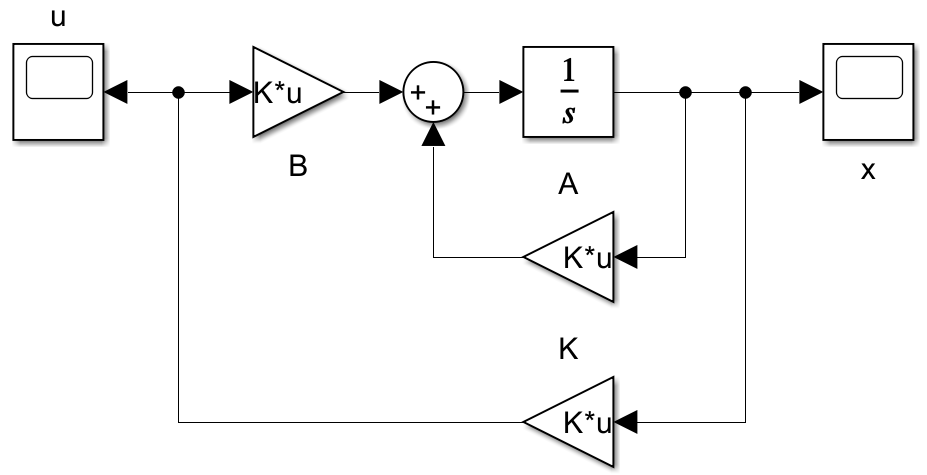
\includegraphics[scale=0.5]{scheme_task1_2.png}
        \captionsetup{skip=0pt}
        \caption{Компьютерное моделирование $u(t),x(t)$}
        \label{fig:scheme_task1_2}
    \end{figure}


    Далее предложены графики $u(t),x(t)$ для каждой матрицы $K_i$
    \begin{figure}[H]
        \centering
        \begin{subfigure}{0.45\textwidth}
            \centering
            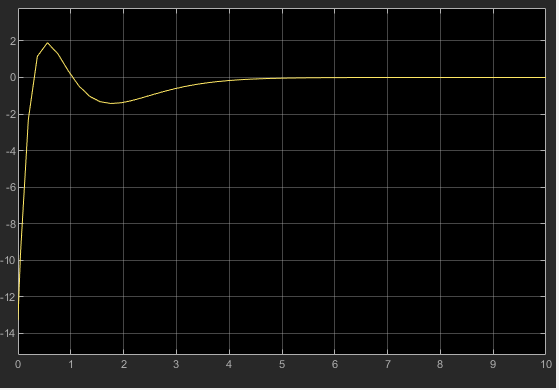
\includegraphics[width=\linewidth]{u_t_k1_task1.png}
            \caption{График $u(t)$}
            \label{fig:task_1_u_t_k1}
        \end{subfigure}
        \hfill
        \begin{subfigure}{0.45\textwidth}
            \centering
            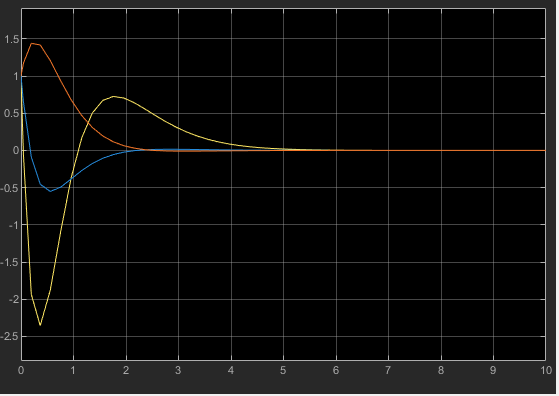
\includegraphics[width=\linewidth]{x_t_k1_task1.png}
            \caption{График $x(t)$}
            \label{fig:task_1_x_t_k1}
        \end{subfigure}
        \caption{Графики $u(t),x(t)$ для $K_1$}
        \label{fig:task_1_modeling_1}
    \end{figure}
    \begin{figure}[H]
        \centering
        \begin{subfigure}{0.45\textwidth}
            \centering
            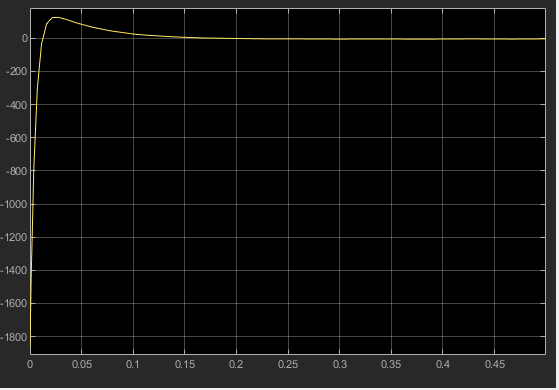
\includegraphics[width=\linewidth]{u_t_k2_task1.png}
            \caption{График $u(t)$}
            \label{fig:task_1_u_t_k2}
        \end{subfigure}
        \hfill
        \begin{subfigure}{0.45\textwidth}
            \centering
            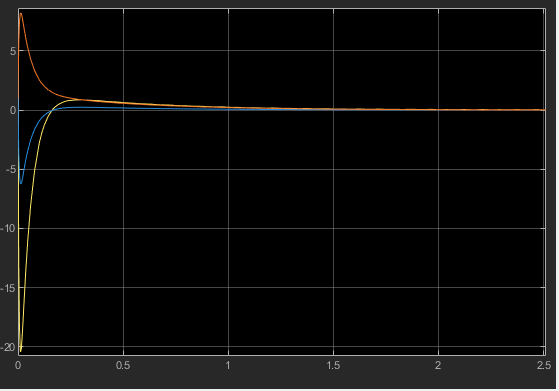
\includegraphics[width=\linewidth]{x_t_k2_task1.png}
            \caption{График $x(t)$}
            \label{fig:task_1_x_t_k2}
        \end{subfigure}
        \caption{Графики $u(t),x(t)$ для $K_2$}
        \label{fig:task_1_modeling_2}
    \end{figure}
    \begin{figure}[H]
        \centering
        \begin{subfigure}{0.45\textwidth}
            \centering
            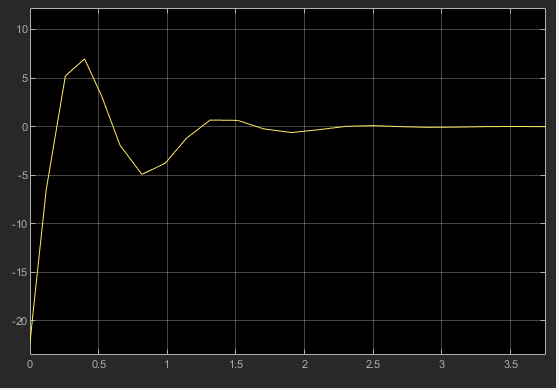
\includegraphics[width=\linewidth]{u_t_k3_task1.png}
            \caption{График $u(t)$}
            \label{fig:task_1_u_t_k3}
        \end{subfigure}
        \hfill
        \begin{subfigure}{0.45\textwidth}
            \centering
            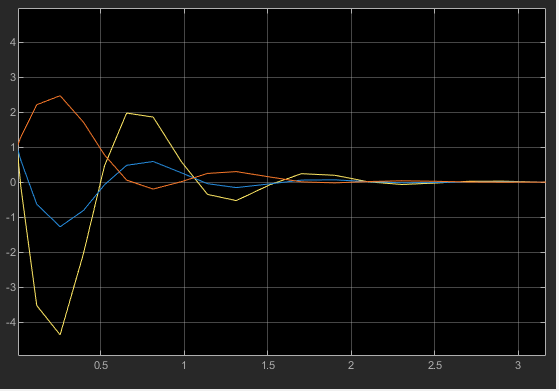
\includegraphics[width=\linewidth]{x_t_k3_task1.png}
            \caption{График $x(t)$}
            \label{fig:task_1_x_t_k3}
        \end{subfigure}
        \caption{Графики $u(t),x(t)$ для $K_3$}
        \label{fig:task_1_modeling_3}
    \end{figure}


    \subsection{Сравнение результатов}
    Сопоставим полученные результаты компьютерного моделирования для рассмотренных спектров,
    оценим возможные сравнительные преимущества и недостатки каждого из них.
    

    ...


    \section{Приложения}
    \subsection{Приложение 1}
    \begin{lstlisting}[label=task1, caption={Программа для первого задания}]
    % input data
    A = [5 2 7; 2 1 2; -2 -3 -4];
    B = [3; 1; -1];

    % A matrix eigenvalues
    A_e = eig(A);
    disp(A_e);

    % Jordan matrix
    [P, J] = jordan(A);
    Pre(:,1) = P(:,1);
    Pre(:,2) = imag(P(:,2));
    Pre(:,3) = real(P(:,3));
    Pre_inv = Pre^-1; 
    J_re = Pre_inv * A * Pre;
    B_jre = Pre_inv * B;
    disp(Pre);
    disp(Pre_inv);
    disp(J_re);
    disp(B_jre);

    % G matrices
    G1 = [0 1 0; 0 0 1; -8 -12 -6];
    Y1 = [1 0 0];
    O1 = [Y1; Y1*G1; Y1*G1^2];
    rank_O1 = rank(O1);
    disp(O1);
    disp(rank_O1);

    G2 = [0 1 0; 0 0 1; -8000 -4440 -222];
    Y2 = [1 0 0];
    O2 = [Y2; Y2*G2; Y2*G2^2];
    rank_O2 = rank(O2);
    disp(O2);
    disp(rank_O2);

    G3 = [0 1 0; 0 0 1; -80 -48 -6];
    Y3 = [1 0 0];
    O3 = [Y3; Y3*G3; Y3*G3^2];
    rank_O3 = rank(O3);
    disp(O3);
    disp(rank_O3);

    % regulator synthesis
    cvx_begin sdp
    variable P1(3,3)
    variable P2(3,3)
    variable P3(3,3)
    A*P1-P1*G1 == B*Y1;
    A*P2-P2*G2 == B*Y2;
    A*P3-P3*G3 == B*Y3;
    cvx_end

    K1 = -Y1*inv(P1);
    disp(P1);
    disp(K1);

    K2 = -Y2*inv(P2);
    disp(P2);
    disp(K2);

    K3 = -Y3*inv(P3);
    disp(P3);
    disp(K3);

    % A+BK eigenvalues
    ABK1 = A+B*K1;
    ABK2 = A+B*K2;
    ABK3 = A+B*K3;

    ABK1_eig = eig(ABK1);
    ABK2_eig = eig(ABK2);
    ABK3_eig = eig(ABK3);

    disp(ABK1);
    disp(ABK1_eig);

    disp(ABK2);
    disp(ABK2_eig);

    disp(ABK3);
    disp(ABK3_eig);
    \end{lstlisting}
\end{document}